\newpage
\section{Geometrical Optics}

\subsection{Plane Mirrors}

\begin{enumerate}
    \item For a point source of light $O$ (object). 
    \begin{figure}[H]
        \centering
        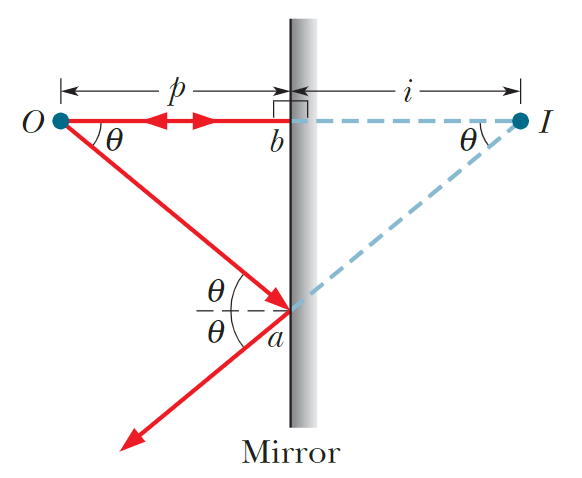
\includegraphics[width=0.309\textwidth]{Lec16/Plane Mirrors}
        \caption{A point source}
    \end{figure}

    $O$ represents object , $I$ represents (virtual) image, $p$ represents object distances (positive quantities), $i$ represents image distances (negative quantities). 
    \begin{align*}
        i=-p
    \end{align*}

    \item For an extended object $O$. 
    \begin{figure}[H]
        \centering
        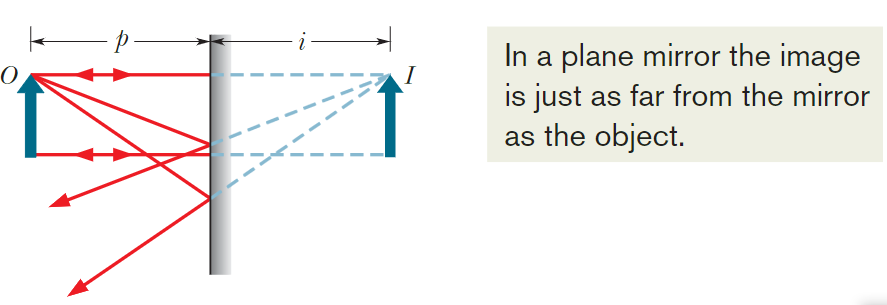
\includegraphics[width=0.309\textwidth]{Lec16/An extended object}
        \caption{An extended object}
    \end{figure}
\end{enumerate}

\subsection{Spherical Mirrors}

\subsubsection[The Concave Mirror and the Convex Mirror]{ The Concave Mirror (凹面镜) and the Convex Mirror (凸面镜)}
\begin{figure}[H]
    \centering
    \begin{minipage}{0.22\textwidth}
        \centering
        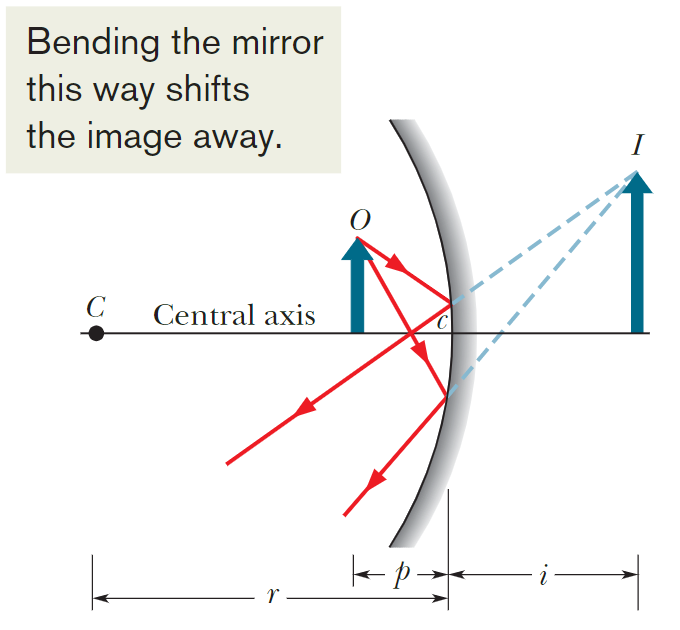
\includegraphics[width=\textwidth]{Lec16/a concave mirror}
        \caption{a concave mirror}
    \end{minipage}
    \begin{minipage}{0.22\textwidth}
        \centering
        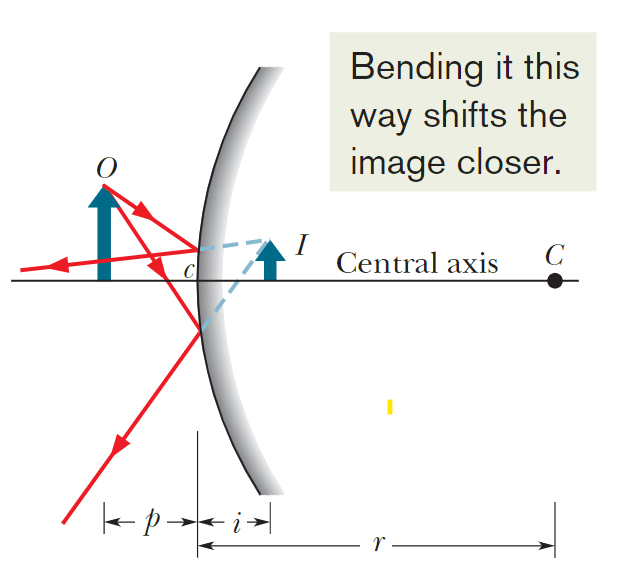
\includegraphics[width=\textwidth]{Lec16/a convex mirror}
        \caption{a convex mirror}
    \end{minipage}
\end{figure}

$C$ represents the center of curvature. 

\subsubsection{Focal Points of Spherical Mirrors}

\begin{figure}[H]
    \centering
    \begin{minipage}{0.22\textwidth}
        \centering
        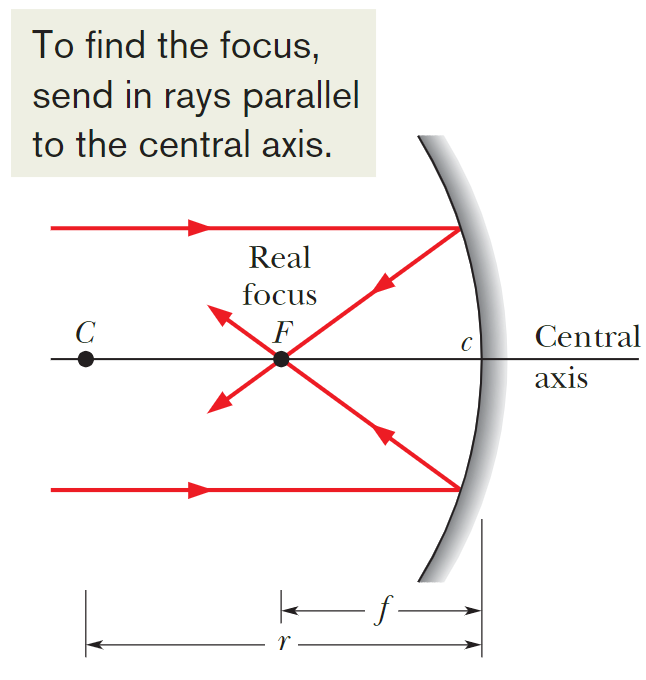
\includegraphics[width=\textwidth]{Lec16/Focal Points of The Concave Mirror}
        \caption{Focal Points of The Concave Mirror}
    \end{minipage}
    \begin{minipage}{0.22\textwidth}
        \centering
        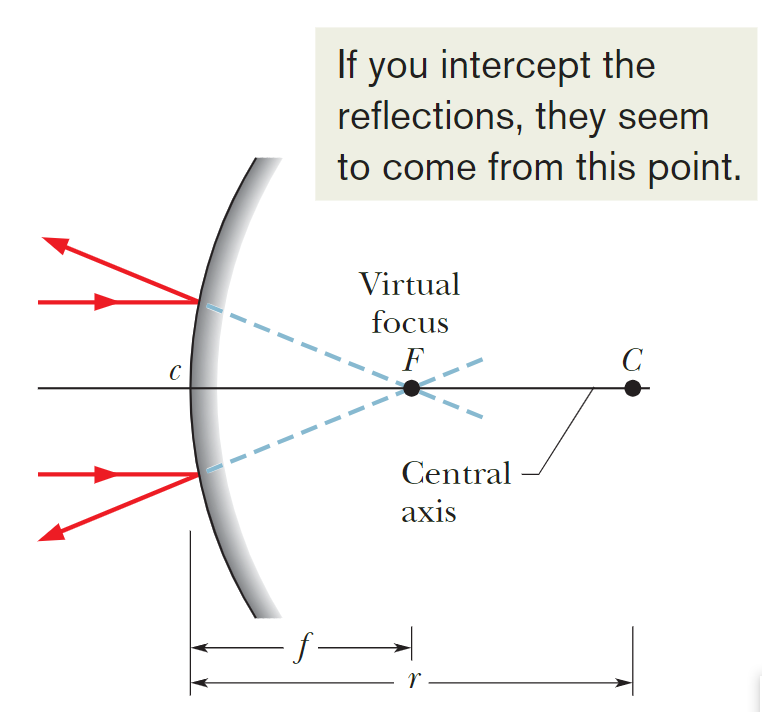
\includegraphics[width=\textwidth]{Lec16/Focal Points of The Convex Mirror}
        \caption{Focal Points of The Convex Mirror}
    \end{minipage}
\end{figure}

\begin{table}[H]
    \centering
    \begin{tabular}[c]{|c|c|c|}\hline
        Mirror type & Concave & Convex\\ \hline
        $F$ & real & virtual \\ 
        $f$ & $f>0$ & $f<0$\\ \hline
    \end{tabular}
    \caption{Mirror types}
\end{table}


$F$ represents the focal point, $f$ represents the focal length, $r$ represents the radius of curvature. 
\begin{align*}
    f=\frac{r }{2}
\end{align*}

Real images form on the side of a mirror where the object is, and virtual images form on the opposite side.

\subsubsection{Images from Spherical Mirrors}

\begin{figure}[H]
    \centering
    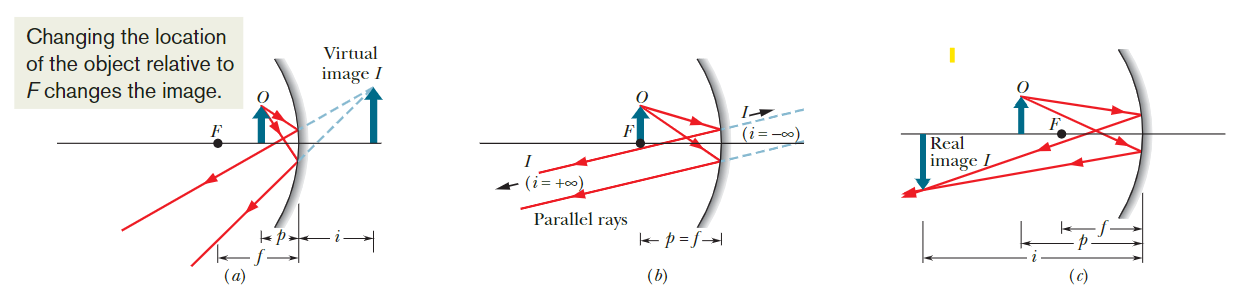
\includegraphics[width=0.48\textwidth]{Lec16/Images from Concave}
    \caption{(a) An object $O$ inside the focal point of a concave mirror, and its virtual image $I$. (b) The object at the focal point $F$ . (c) The object outside the focal point, and its real image $I$.}
\end{figure}

\begin{align*}
    \frac{1}{p }+\frac{1 }{i }=\frac{1 }{f }
\end{align*}

\begin{enumerate}
    \item The angles should be small. 
    \item The equation applies to any concave $(f > 0)$, convex $(f < 0)$, or plane $(f = \infty )$ mirror.
    \item For a convex or plane mirror, only a virtual image can be formed, regardless of the object’s location on the central axis.
\end{enumerate}

Rules to locate an image: 
\begin{enumerate}
    \item A ray that is initially parallel to the
    central axis reflects through the focal point F . 
    \item A ray that reflects from the mirror after passing through the focal point emerges parallel to the central axis. 
    \item A ray that reflects from the mirror after passing through the center of curvature C returns along itself. 
    \item A ray that reflects from the mirror at point c is reflected symmetrically about that axis.
\end{enumerate}

\begin{figure}[H]
    \centering
    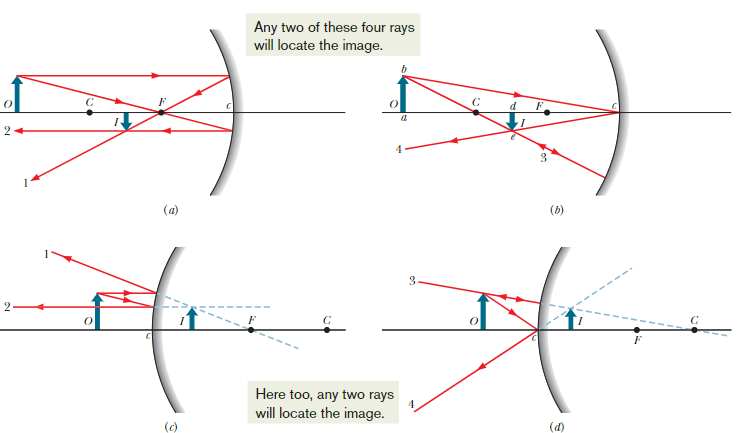
\includegraphics[width=0.47\textwidth]{Lec16/Rules to locate an image}
    \caption{Rules to locate an image}
\end{figure}

$h$ represents the height of the object, $h^{\prime}$ represents the height of the image. $m$ is called the \highlight{lateral magnification (横倍率)} produced by the mirror. 

\begin{align*}
    m \equiv \frac{h^{\prime}}{h} = -\frac{i}{p} 
\end{align*}

\subsection{Spherical Refraction}

For light rays making only small angles with the central axis, so $\sin\theta\sim\theta$. 
\begin{align*}
    \frac{n_1}{p}+\frac{n_2}{i}=\frac{n_2-n_1}{2f}=\frac{n_2-n_1}{r}
\end{align*}

\begin{figure}[H]
    \centering
    \begin{subfigure}{0.309\textwidth}
        \centering
        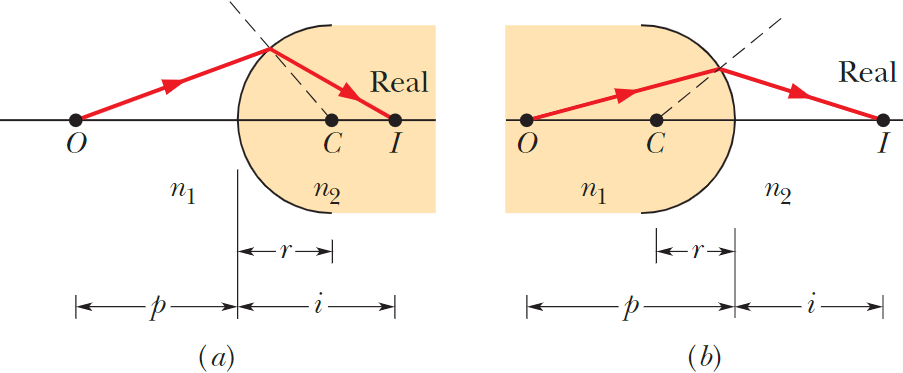
\includegraphics[width=\textwidth]{Lec16/Spherical Refraction 1}
    \end{subfigure}

    \begin{subfigure}{0.309\textwidth}
        \centering
        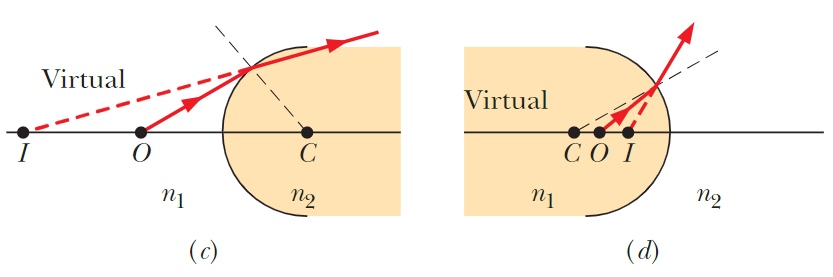
\includegraphics[width=\textwidth]{Lec16/Spherical Refraction 2}
    \end{subfigure}

    \begin{subfigure}{0.309\textwidth}
        \centering
        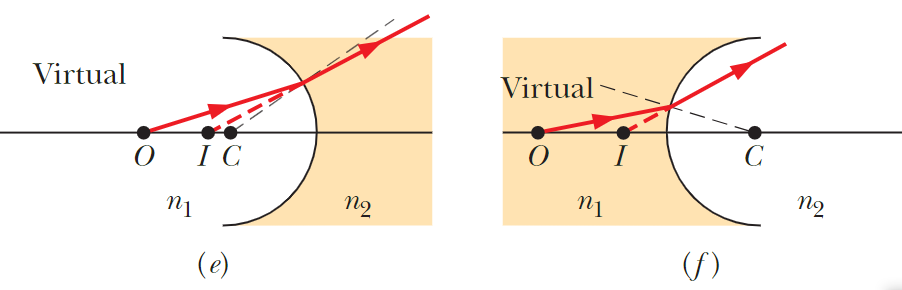
\includegraphics[width=\textwidth]{Lec16/Spherical Refraction 3}
    \end{subfigure}

    \caption{Spherical Refraction}
\end{figure}


\subsection{Thin Lenses}
A \highlight{lens} is a transparent object with two refracting surfaces whose central axes coincide.

A lens that causes light rays initially parallel to the central axis to converge is (reasonably) called a \highlight{converging lens (汇聚透镜)}. If, instead, it causes such rays to diverge, the lens is a \highlight{diverging lens (发散透镜)}.

We consider a \highlight{thin lens}, i.e., a lens in which the thickest part is thin relative to the object distance $p$, the image distance $i$, and the radii of curvature $r_1$ and $r_2$ of the two surfaces of the lens.

We also consider only light rays that make small angles with the central axis (again, they are exaggerated in the figures).

\begin{figure}[H]
    \centering
    \begin{minipage}{0.309\textwidth}
        \centering
        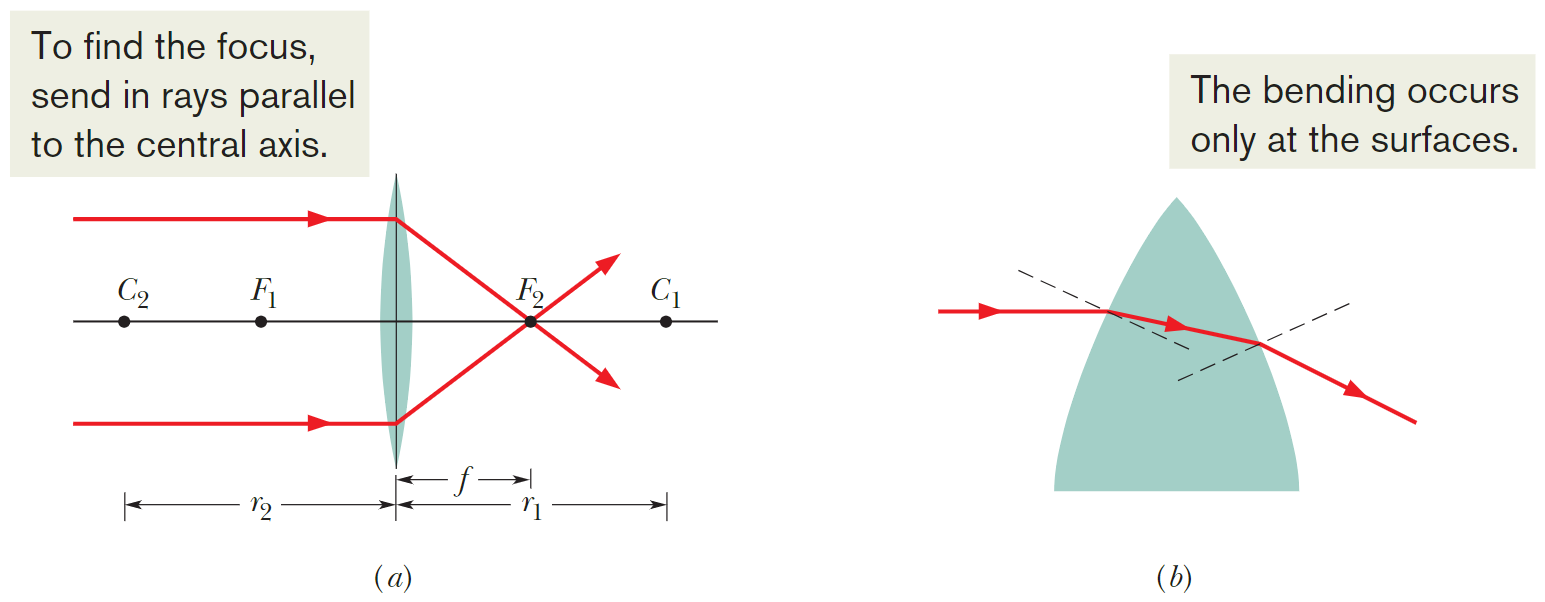
\includegraphics[width=\textwidth]{Lec16/converging lens}
        \caption{converging lens}
    \end{minipage}

    \begin{minipage}{0.309\textwidth}
        \centering
        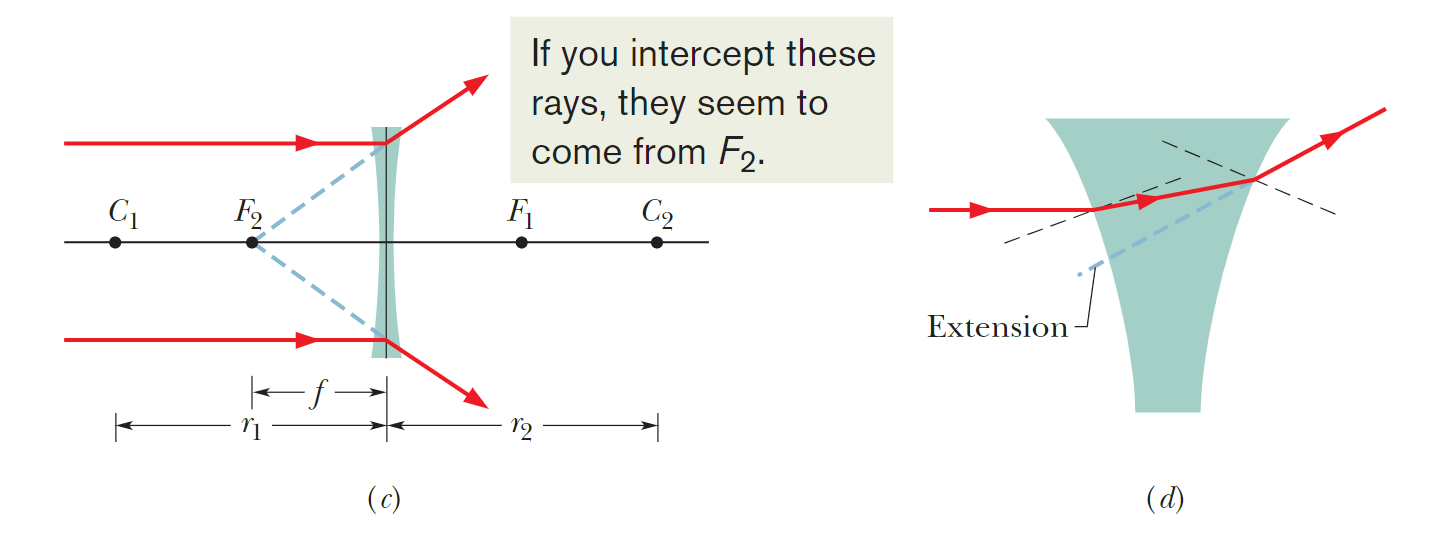
\includegraphics[width=\textwidth]{Lec16/diverging lens}
        \caption{diverging lens}
    \end{minipage}
\end{figure}

When a thin lens with index of refraction n is surrounded by air, this focal length $f$ is given by the \highlight{lens maker’s equation}: 
\begin{align*}
    \frac{1}{f }=(n-1)\left( \frac{1}{r_1}-\frac{1}{r_2} \right)
\end{align*}

If the lens is surrounded by some medium other than air (say,
corn oil) with index of refraction $n_{medium}$, we replace $n$ with
$\frac{n}{n_{medium}}$.

For a thin lens with a focal length $f$ , $i$ and $p$ are related to each other by
\begin{align*}
    \frac{1}{p}+\frac{1}{i}=\frac{1}{f}
\end{align*}

\begin{enumerate}
    \item A ray that is initially parallel to the central axis of the lens will pass through focal point $F_2$. 
    \item A ray that initially passes through focal point $F_1$ will emerge from the lens parallel to the central axis.
    \item A ray that is initially directed toward the center of the lens will emerge from the lens with no change in its direction because the ray encounters the two sides of the lens where they are almost parallel.
\end{enumerate}

\subsection{Lens Systems} 
\subsubsection{Combination of Thin Lenses}
We treat the two-lens system with two single-lens calculations, using the normal rules for a single len. The overall (or net) lateral magnification $M$ of a system of lenses (or lenses and a mirror) is the product of the individual lateral magnifications. 

\subsubsection{Compound Microscope}
A compound microscope consists of an objective (the front lens) of focal length $f_{ob}$ and an eyepiece (the lens near the eye) of focal length $f_{ey}$. So we generate the virtual image of a real image of the
object. We want both images being magnified. 
\begin{figure}[H]
    \centering
    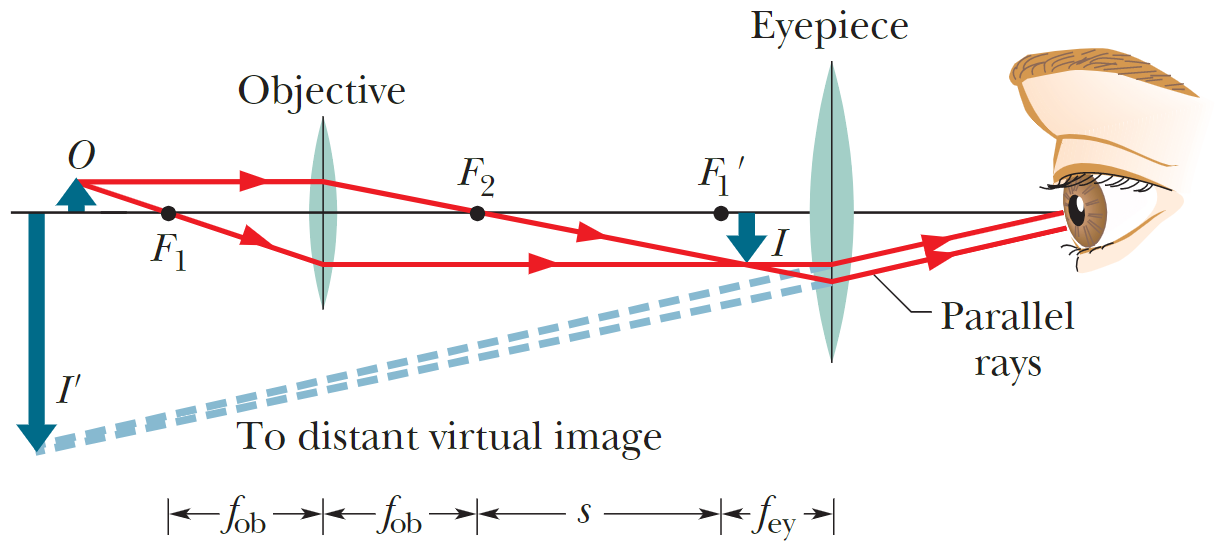
\includegraphics[width=0.309\textwidth]{Lec16/Compound Microscope}
    \caption{Compound Microscope}
\end{figure}

For the objective, we want the image to be magnified, so $i_1\gg p_1$. This can be satisfied by setting $p_1 \gtrsim f_{ob}$.

For the eyepiece, we expect $p_2\lesssim f_{ey}$. 

This leaves the distance between the two lenses
$f_{ob} + s + f_{ey}$ the only parameter to tune. The longer the distance, the larger the magnification
\begin{align*}
    M=m_1m_2\approx -\frac{\left(f_{ob}+s \right)}{f_{ob}}\frac{25 \mathrm{cm}}{f_{ey}}
\end{align*}

We can make $s \gg f_{ob}$, so
\begin{align*}
    M\approx -\frac{s}{f_{ob}}\frac{25\mathrm{cm}}{f_{ey}}
\end{align*}

But $s$ is still limited by the practical sizes of the microscope. 